\documentclass{mwart}
%\usepackage{polski}
%\usepackage[polish]{babel}
\usepackage{amsfonts}
\usepackage{indentfirst}
\usepackage[utf8]{inputenc}
\usepackage{amsthm}
\usepackage{multirow}
\usepackage{amsmath}
\newtheorem{tw}{Twierdzenie}
\newtheorem{df}{Definicja}
\newtheorem{zd}{Zadanie}
\newtheorem{zdt}[zd]{Zadanie*}
\title{Procesy stochastyczne\\ Zestaw zadań nr 6}
\usepackage{Sweave}
\begin{document}
\Sconcordance{concordance:Zestaw6_PS_2020.tex:Zestaw6_PS_2020.Rnw:%
1 14 1 1 0 33 1 1 25 1 2 1 1}

\maketitle
\begin{zd}
	Niech $N_t$ będzie procesem Poissona z intensywnością $\lambda$. Udowodnij
	\begin{displaymath}
	\lim_{t\to \infty}\frac{N_t}{t} = \lambda\ p.n.
	\end{displaymath}
\end{zd}
\begin{zd}
	Udowodnij, że suma niezależnych procesów Poissona jest procesem Poissona. Jaką intesywność ma otrzymany proces?
\end{zd}
\begin{zd}
Niech $N_t$ będzie procesem Poissona z intensywnością $\lambda$. Znajdź postać funkcji kowariancji tego procesu
\begin{displaymath}
C_N(t,s) = Cov(N_t, N_s)
\end{displaymath}
oraz funkcję autokorelacji tego procesu
\begin{displaymath}
	A_N(t,s) = \rho\left(N_t, N_s\right).
\end{displaymath}
\end{zd}
\begin{zd}
	Niech $N_t$ będzie procesem Poissona z intensywnością $\lambda$ i niech $X_1$ będzie czasem pierwszego przybycia. Pokaż, że warunkowo względem zdarzenia $N(t) = 1$, $X_1$ ma rozkład jednostajny na odcinku $(0,t]$, czyli
	\begin{displaymath}
	\mathbb{P}\left(X_1 \leq x|N(t) = 1\right) = \frac{x}{t},\ 0\leq x\leq t.
	\end{displaymath}
\end{zd}
\begin{zd}
Udowodnij, że jednorodny proces Poissona ma własność Markowa.
\end{zd}
\begin{zd}
Niech $N$ będzie jednorodnym procesem Poissona z intensywnością $\lambda$. Dla pewnego $s>0$ określmy $\tilde{N}_t = N_{t+s} - N_s$. Udowodnij, że $\tilde{N}$ jest procesem Poissona z tą samą intensywnością $\lambda$.
\end{zd}
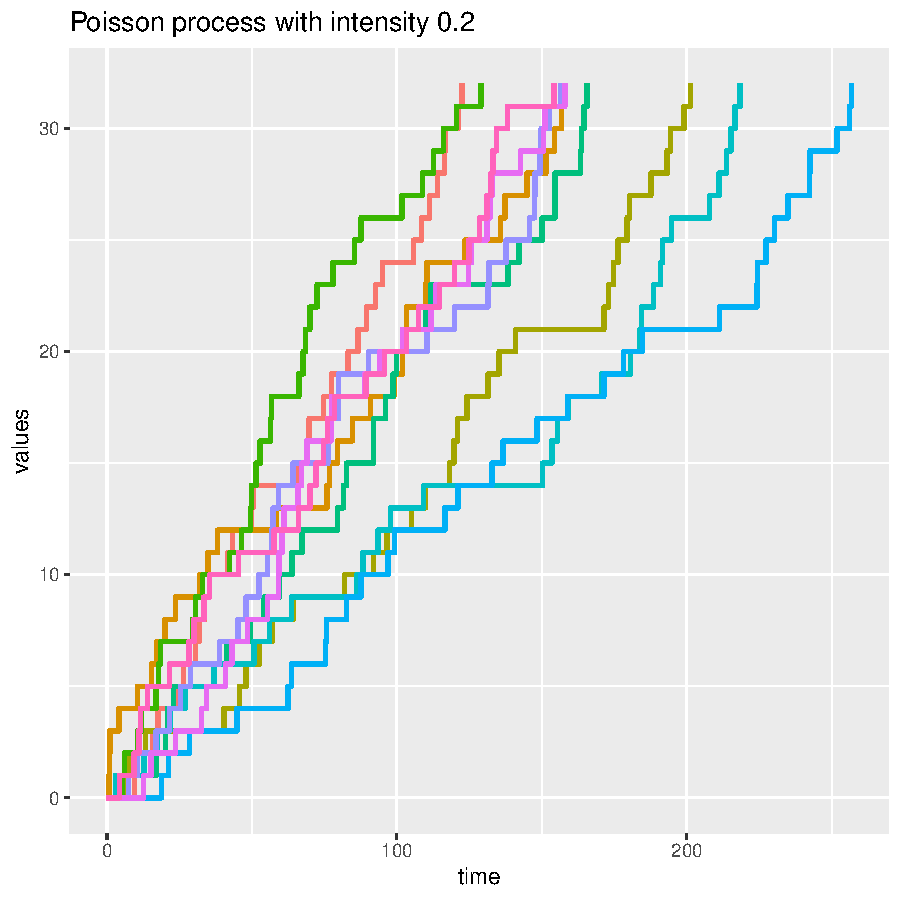
\includegraphics{Zestaw6_PS_2020-001}

\end{document}
